\documentclass[tikz,border=10pt]{standalone}
\usepackage{tikz}
\usetikzlibrary{arrows.meta}

\begin{document}
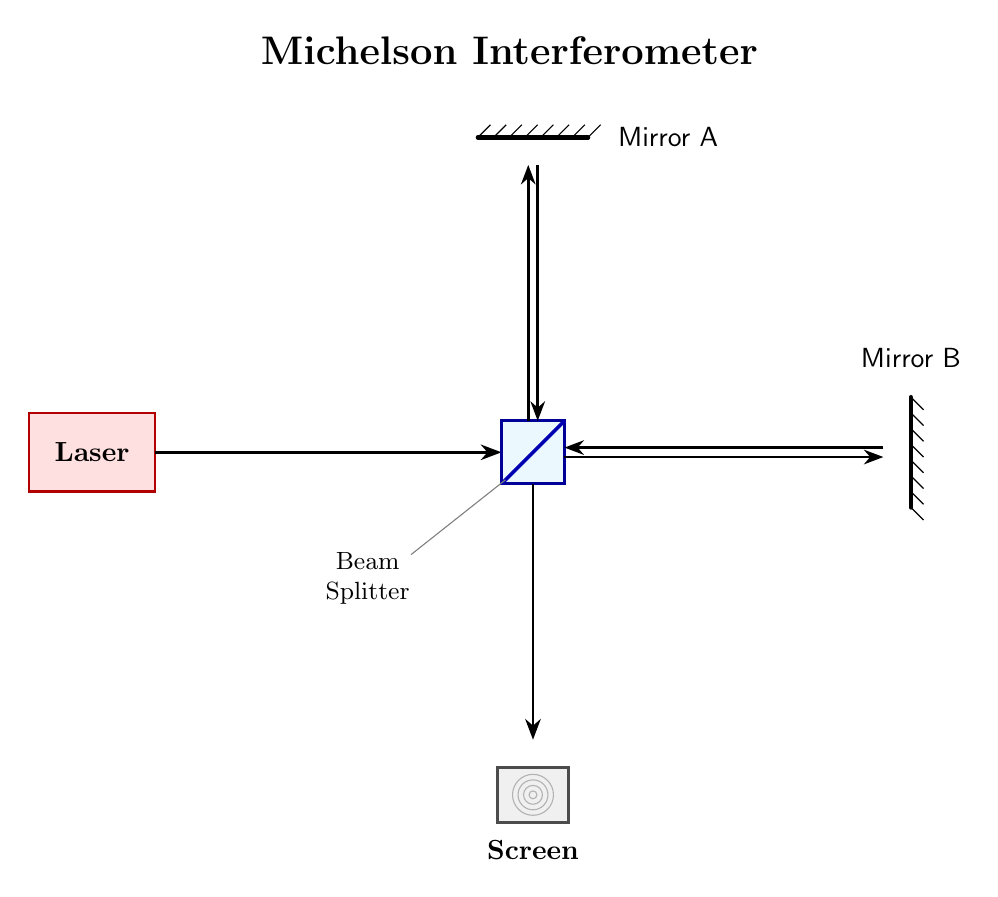
\begin{tikzpicture}[
  >=Stealth,
  every node/.style={font=\sffamily},
  thick
]

% ============================================================
% Title
% ============================================================
\node[font=\Large\bfseries] at (-0.3,5.1) {Michelson Interferometer};

% ============================================================
% Laser
% ============================================================
\draw[draw=red!70!black, fill=red!12, line width=1pt]
  (-6.4,-0.5) rectangle (-4.8,0.5);
\node[font=\bfseries] at (-5.6,0) {Laser};

% Beam: Laser -> Beam Splitter (single incoming beam)
\draw[->, line width=1pt] (-4.8,0) -- (-0.4,0);

% ============================================================
% Beam Splitter (square block with 45-degree splitting surface)
% ============================================================
\draw[draw=blue!60!black, fill=cyan!8, line width=1pt]
  (-0.4,-0.4) rectangle (0.4,0.4);
\draw[draw=blue!70!black, line width=1.3pt] (-0.4,-0.4) -- (0.4,0.4);

\node[align=center, font=\small] at (-2.1,-1.6) {Beam\\Splitter};
\draw[gray, thin] (-1.55,-1.3) -- (-0.35,-0.35);

% ============================================================
% Arm to Mirror A (up) — outgoing + returning beams
% ============================================================
\draw[->, line width=0.9pt] (-0.06,0.4) -- (-0.06,3.65);
\draw[->, line width=0.9pt] (0.06,3.65) -- (0.06,0.4);

% Mirror A
\draw[line width=1.6pt, line cap=round] (-0.7,4) -- (0.7,4);
\foreach \x in {-0.7,-0.5,-0.3,-0.1,0.1,0.3,0.5,0.7} {
  \draw[thin] (\x,4) -- ++(0.16,0.16);
}
\node[anchor=west] at (0.95,4) {Mirror A};

% ============================================================
% Arm to Mirror B (right) — outgoing + returning beams
% ============================================================
\draw[->, line width=0.9pt] (0.4,-0.06) -- (4.45,-0.06);
\draw[->, line width=0.9pt] (4.45,0.06) -- (0.4,0.06);

% Mirror B
\draw[line width=1.6pt, line cap=round] (4.8,-0.7) -- (4.8,0.7);
\foreach \y in {-0.7,-0.5,-0.3,-0.1,0.1,0.3,0.5,0.7} {
  \draw[thin] (4.8,\y) -- ++(0.16,-0.16);
}
\node[anchor=south] at (4.8,0.95) {Mirror B};

% ============================================================
% Beam: Beam Splitter -> Screen (recombined output beam)
% ============================================================
\draw[->, line width=1pt] (0,-0.4) -- (0,-3.65);

% ============================================================
% Screen
% ============================================================
\draw[draw=gray!60!black, fill=gray!12, line width=1pt]
  (-0.45,-4.7) rectangle (0.45,-4.0);
\foreach \r in {0.05,0.12,0.19,0.26} {
  \draw[gray!60, thin] (0,-4.35) circle (\r cm);
}
\node[font=\bfseries] at (0,-5.05) {Screen};

\end{tikzpicture}
\end{document}
